%!TEX root = ../template.tex
%%%%%%%%%%%%%%%%%%%%%%%%%%%%%%%%%%%%%%%%%%%%%%%%%%%%%%%%%%%%%%%%%%%%
%% chapter2.tex
%% NOVA thesis document file
%%
%% Chapter with the template manual
%%%%%%%%%%%%%%%%%%%%%%%%%%%%%%%%%%%%%%%%%%%%%%%%%%%%%%%%%%%%%%%%%%%%

\typeout{NT FILE chapter2.tex}%

\chapter{Theoretical Framework: Complexity and Efficiency}\label{chapt:2}
% \Glsresetall



\section{Computational Complexity}

Computational complexity refers to the study of resource requirements of algorithms, focusing primarily on time and space resources as a function of input size. This field categorizes problems based on the minimum resources needed to solve them, providing a theoretical framework for understanding the intrinsic difficulty of computational problems and the efficiency of algorithms designed to solve them. ~\cite{GareyJohnson1979}

\subsection{Time Complexity}

Time complexity is a measure of the amount of computational time an algorithm takes to complete as a function of the input length. It is often expressed using Big O notation, which describes the upper bound of the growth rate of execution time ~\cite{BigONotation}. Understanding the time complexity of an algorithm is crucial for predicting its scalability and feasibility in practical applications, especially for problems known to be computationally intensive such as the \Gls{TSP}.

The \Gls{TSP}, being \Gls{NP}-hard, does not have a known polynomial-time solution that can efficiently solve all instances of the problem. The brute-force approach for the \Gls{TSP}, for example, has a factorial time complexity (\(O(n!)\)), making it computationally infeasible even for moderately large problem instances. This has led to the exploration of various heuristic and metaheuristic algorithms that aim for acceptable solutions in polynomial time (\(O(n^k)\)), where \(k\) is a constant, trading accuracy for efficiency and practical applicability.~\cite{Dorigo1996}


\begin{figure}[h]
	\centering
	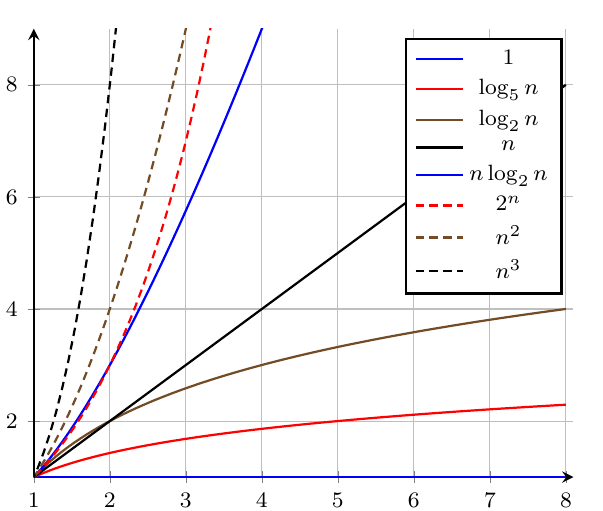
\begin{tikzpicture}
		\begin{axis}
			[
				axis lines = left,
				xmin=1, xmax=8.1, ymin=1, ymax=9,
				domain=0:8, samples=100, no markers, thick, grid=both,
				xlabel = \(n\), ylabel = {\(f(n)\)},
				label style = {overlay},       % Has he same effect as
				ticklabel style = {overlay},   % trim axis [left|right]
				legend entries = {
						$1$,
						$\log_{5}n$,
						$\log_{2}n$,
						$n$,
						$n\log_{2}n$,
						$2^{n}$,
						$n^{2}$,
						$n^{3}$,
					},
				every axis/.style = {font=\footnotesize},
				label style = {font=\normalsize},
			]
			\addplot+ {1};
			\addplot+ {1 + ln(x)/ln(5)};
			\addplot+ {1 + ln(x)/ln(2)};
			\addplot+ {x};
			\addplot+ {1 + x*ln(x)/ln(2)};
			\addplot+ {2^x-1};
			\addplot+ {x^2};
			\addplot+ {x^3};
		\end{axis}
	\end{tikzpicture}
	\vspace{1.0cm}
	\caption{Growth rate of different complexities}
\end{figure}


\begin{table}[h]
	\centering
	\caption{Number of possible permutations per number of cities}
	\begin{tabular}{c l}
		\toprule
		Number of cities & Number of Permutations                \\
		\midrule
		4            & 24                                 \\
		5            & 120                                \\
		6            & 720                                \\
		7            & 5,040                              \\
		8            & 40,320                             \\
		9            & 362,880                            \\
		10           & 3,628,800                          \\
		11           & 39,916,800                         \\
		12           & 479,001,600                        \\
		13           & 6,227,020,800                      \\
		14           & 87,178,291,200                     \\
		15           & 1,307,674,368,000                  \\
		16           & 20,922,789,888,000                 \\
		17           & 355,687,428,096,000                \\
		18           & 6,402,373,705,728,000              \\
		19           & 121,645,100,408,832,000            \\
		20           & 2,432,902,008,176,640,000          \\
		25           & 15,511,210,043,330,985,984,000,000 \\
		\bottomrule
	\end{tabular}
\end{table}

\subsection{Space Complexity}

Space complexity measures the total amount of memory an algorithm requires as a function of input size. Like time complexity, space complexity is crucial for evaluating the efficiency of an algorithm, particularly in scenarios where memory resources are limited. In the context of the \Gls{TSP} and similar optimization problems, the space complexity of an algorithm can significantly impact its usability in real-world applications, where solutions often need to be computed in real-time or on hardware with limited memory capacity.~\cite{HeldKarp1962}.

For example, dynamic programming approaches for the \Gls{TSP}, such as the Held-Karp algorithm, offer a more favorable time complexity compared to brute force (\(O(n^2 2^n)\)) but at the cost of exponential space complexity (\(O(n^2)\)). Such trade-offs between time and space complexity are central considerations in algorithm design, especially when developing new algorithms intended for large-scale problem instances, such as those encountered in logistics and routing applications.

\section{The \Gls{P} vs. \Gls{NP} Problem}

The \Gls{P} vs \Gls{NP} problem represents one of the most significant open questions in the field of theoretical computer science. It concerns establishing whether every problem whose solution can be efficiently verified (in polynomial time) by a computer can also be solved just as quickly (also in polynomial time). The \Gls{P} class includes problems that can be solved quickly, while the \Gls{NP} class comprises problems for which a given solution can be verified quickly.~\cite{PvsNP}.
\begin{figure}[h]
	\centering
	% TODO: Use venndiagram package to draw the diagram
	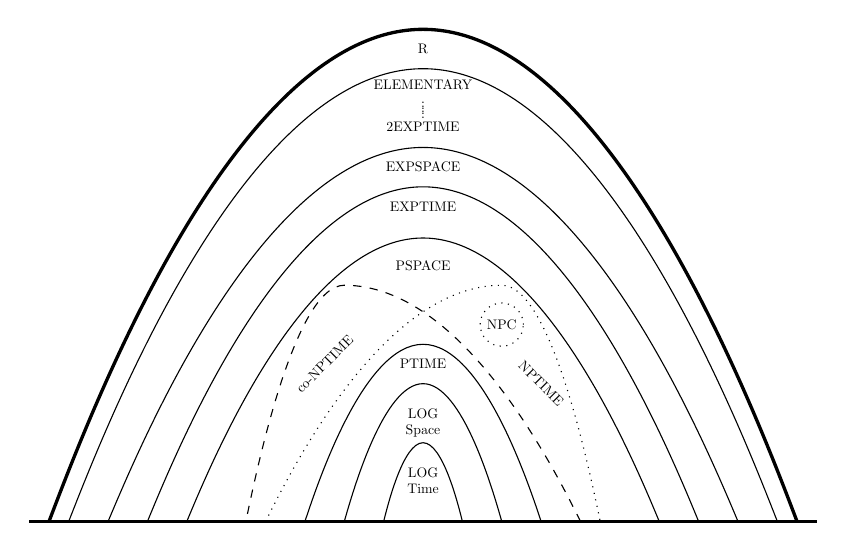
\begin{tikzpicture}[scale=0.5, every node/.append style={scale=0.5}]
		\pgftransformscale{1}

		%%% HELP LINES - uncomment to design/extend
		% \draw[step=1cm,gray,very thin] (-10,0) grid (10,12);
		% \node at (0,0) {\textbf{(0,0)}};

		%% Horizontal bar
		\draw[very thick] (10,0) -- (-10,0);

		% LOG TIME
		\draw (-1,0) parabola bend (0,2) (1,0) ;
		\node at (0,1) {
			\begin{tabular}{c}
				LOG \\ Time
			\end{tabular}
		};

		% LOG SPACE
		\draw (-2,0) parabola bend (0,3.5) (2,0);
		\node at (0,2.5) {
			\begin{tabular}{c}
				LOG \\ Space
			\end{tabular}
		};

		% PTIME
		\draw (-3,0) parabola bend (0,4.5) (3,0);
		\node at (0,4) {PTIME};

		% NP
		\draw[dotted] (-4,0) parabola bend (2,6) (4.5,0);
		\node[rotate=-45] at (3,3.5) {NPTIME};

		% NP-complete
		\node[circle,dotted,draw] at (2,5) {NPC};

		% Co-NP
		\draw[dashed] (4,0) parabola bend (-2,6) (-4.5,0);
		\node[rotate=45] at (-2.5,4) {co-NPTIME};

		% PSPACE
		\draw (-6,0) parabola bend (0,7.2) (6,0);
		\node at (0,6.5) {PSPACE};

		% EXPTIME
		\draw (-7,0) parabola bend (0,8.5) (7,0);
		\node at (0,8) {EXPTIME};

		% EXPTIME
		\draw (-8,0) parabola bend (0,9.5) (8,0);
		\node at (0,9) {EXPSPACE};

		% ELEMENTARY
		\draw (-9,0) parabola bend (0,11.5) (9,0);
		\node at (0,10.5) {$\vdots$};
		\node[anchor=north] at (0,11.4) {
			\begin{tabular}{c}
				ELEMENTARY \\
				$\vdots$   \\
				2EXPTIME
			\end{tabular}
		};

		% RECURSIVE
		\draw[very thick] (-9.5,0) parabola bend (0,12.5) (9.5,0);
		\node at (0,12) {R};
	\end{tikzpicture}
	\caption{Classification of computational problems}
\end{figure}
\subsection{Definition and Relevance}

Formally, a problem belongs to the \Gls{P} class if it can be solved in polynomial time, which means that the amount of time needed to solve the problem grows polynomially with the size of the input. The \Gls{NP} class, on the other hand, comprises problems for which a given solution can be verified in polynomial time. The \Gls{P} vs. \Gls{NP} problem essentially asks whether these two classes are equal; that is, whether every problem that can be verified quickly can also be solved quickly.

The relevance of the \Gls{P} vs. \Gls{NP} problem lies in its implications for a vast field of disciplines, from cryptography and algorithm design to decision-making processes and beyond. A proof that \Gls{P} equals \Gls{NP} could potentially revolutionize the fields of mathematics and computer science, enabling efficient solutions to a multitude of complex problems currently considered intractable. Conversely, proving that \Gls{P} does not equal \Gls{NP} would formalize the intrinsic computational difficulty of these problems.

\subsection{Implications for the \Gls{TSP}}

The classification of the \Gls{TSP} as \Gls{NP}-hard underscores the complexity and computational challenges associated with finding an exact solution for large problem instances. This classification has significant implications for both theoretical research and practical applications in the field. It implies that unless \Gls{P} equals \Gls{NP}, one should not expect to discover an algorithm capable of solving quickly (in polynomial time) and accurately every instance of the \Gls{TSP}. This awareness has shifted the focus of much of the research on the \Gls{TSP} toward the development of heuristic and metaheuristic algorithms, which aim to find sufficiently good solutions in a reasonable time frame, rather than pursuing the elusive goal of an exact solution for all possible instances.~\cite{Karp1972}.

Furthermore, the implications of the \Gls{TSP} being \Gls{NP}-hard extend beyond algorithm development. It influences how problems are modeled in practical scenarios where TSP-like problems arise, such as logistics and routing, network design, and scheduling. In these applications, the emphasis is often on finding solutions that approximate the optimal but can be obtained much more quickly than an exact algorithm would allow. This approach enables industry to achieve efficiency and cost savings even when facing complex routing and scheduling problems.

Therefore, the implications of the \Gls{TSP} classification resonate in both the academic study of algorithm theory and in practical considerations on applying these theories in real-world situations.

\section{Complexity of the \Gls{TSP}}

The proof that the \Gls{TSP} is \Gls{NP}-hard was first presented by Richard M. Karp in 1972. Karp's work, part of a paper that identified 21 \Gls{NP}-complete problems, laid the foundation for understanding the computational limits of algorithmic solutions for the \Gls{TSP} and similar problems. By demonstrating that the decision version of the \Gls{TSP} (determining whether a tour of a given length or less exists) is \Gls{NP}-complete, Karp showed that the optimization version of the \Gls{TSP}, where the goal is to find the shortest possible tour, is \Gls{NP}-hard.

Karp's proof employs a technique known as reduction, in which a known \Gls{NP}-complete problem is transformed into an instance of the \Gls{TSP} in polynomial time. This method illustrates that if a polynomial-time algorithm could solve the \Gls{TSP}, it could, by extension, solve all problems in \Gls{NP}, a proposition that remains unverified. 


\begin{table}[htbp]
	\centering
	\tiny
	\setlength{\tabcolsep}{4pt}
	\begin{tabular*}{\textwidth}{@{\extracolsep{\fill}}p{2cm}p{2cm}p{2cm}p{3.5cm}p{3cm}p{2.5cm}@{}}
			\toprule
			\textbf{Algorithm} & \textbf{Time - Space Complexity} & \textbf{Description} & \textbf{Advantages} & \textbf{Disadvantages} \\ \midrule
			Held-Karp & \(O(n^2 2^n)\) - \(O(n^2)\) & Exact algorithm using dynamic programming & Provides optimal solution & Infeasible for large \(n\) \\[6pt]
			Nearest Neighbor & \(O(n^2)\) - \(O(n)\) & Greedy heuristic algorithm & Simple and fast & Often far from optimal \\[6pt]
			Christofides & \(O(n^3)\) - \(O(n^2)\) & Approximation algorithm with 3/2 ratio & Best approximation for metric TSP & Still not exact \\[6pt]
			Genetic Algorithms & \(O(n^2)\) - \(O(n)\) & Metaheuristic algorithm inspired by natural selection & Flexible and adaptable & No guarantee of optimal solution \\ \bottomrule
	\end{tabular*}
	\caption{Comparison between different algorithms for TSP}
\end{table}

\subsection{Impact on Algorithm Design}

The \Gls{NP}-hardness of the \Gls{TSP} has a profound impact on the design of algorithms to solve it, fostering the development of various strategies aimed at overcoming computational obstacles:

\begin{itemize}
	\item \textbf{Exact algorithms:} Despite the \Gls{NP}-hardness of the \Gls{TSP}, exact algorithms have been devised, such as the Held-Karp algorithm. These algorithms guarantee an optimal solution, but do so at a computational cost that increases exponentially with problem size, making them impractical for large instances.
	\item \textbf{Heuristic approaches:} To tackle larger \Gls{TSP} instances, heuristic algorithms are employed. These algorithms do not guarantee an optimal solution, but can often find good solutions in a fraction of the time required by exact methods. Examples include the Nearest Neighbor algorithm and Christofides' algorithm.
  \item \textbf{Metaheuristic algorithms:} For even more complex instances, metaheuristic approaches, such as the Genetic Algorithm \Gls{GA} and the Ant Colony System \Gls{ACS}, offer flexible strategies that explore the solution space more broadly, aiming to escape local optima and approach global optima more effectively. These techniques draw inspiration from natural processes and have the advantage of adaptability to different problem instances.
\end{itemize}
